\documentclass{emulateapj}

\usepackage[intlimits]{amsmath}
\usepackage{amsthm}
\usepackage{amssymb}
\usepackage{cancel} 
\usepackage{graphicx}
\usepackage{mdwlist}
\usepackage{hyperref}
\usepackage{color}
%\citestyle{aa}

\providecommand{\e}[1]{\times10^{#1}}
\providecommand{\units}[1]{\;\mathrm{#1}}
\providecommand{\diff}[2]{\frac{\partial #1}{\partial #2}}
\providecommand{\ddiff}[2]{\frac{\partial^2 #1}{\partial #2^2}}
\providecommand{\tdiff}[2]{\frac{\mathrm{d} #1}{\mathrm{d} #2}}
\providecommand{\infint}[2]{\int\limits_{-\infty}^{\infty}{#1}\;\mathrm{d}#2} 
\providecommand{\MAA}{\text{\AA}}
\providecommand{\abs}[1]{\left| #1 \right|} % for absolute value
\providecommand{\avg}[1]{\left< #1 \right>} % for average
\providecommand{\grad}[1]{\gv{\nabla} #1} % for gradient
\let\divsymb=\div 
\renewcommand{\div}[1]{\gv{\nabla} \cdot #1} % for divergence
\providecommand{\curl}[1]{\gv{\nabla} \times #1} % for curl
\providecommand{\MAA}{\text{\AA}}

\newcommand\numberthis{\addtocounter{equation}{1}\tag{\theequation}}
\numberwithin{equation}{section}

\providecommand{\MJ}{\ensuremath{\units{M_J}}}
\providecommand{\RJ}{\ensuremath{\units{R_J}}}
\providecommand{\MS}{\ensuremath{\units{M_\odot}}}
\providecommand{\RS}{\ensuremath{\units{R_\odot}}}

\shorttitle{Detecting Extra-Solar Planets}
\shortauthors{Tom Badran}

\begin{document}

\title{Detecting Extra-Solar Planets}
\author{Tom Badran\altaffilmark{1}}
\email{badrant@cardiff.ac.uk}
\affiliation{Cardiff School of Physics and Astronomy}
\altaffiltext{1}{Cardiff School of Physics and Astronomy, Cardiff University, Queens Buildings, The Parade, Cardiff, Wales, CF24 3AA, UK}
\date{September 2013 to May 2014}

\begin{abstract}
%!TEX root = project.tex
Since 1995 many extra solar planets have been discovered using the transit method. I have shown that it is possible to detect these planets using relatively low powered ground based optical telescopes (<0.5m), even under very poor seeing conditions. I also present an algorithm for analysing images and a computer program implementation of this algorithm, including an automated pipeline for processing a large sequence of images. Using this computer program, it was determined that the dwarf star, Hat P 20, has a planet of radius $(0.91\pm0.14) R_J$.

\end{abstract}

\section{Introduction}
%!TEX root = project.tex
\subsection{Motivations}

Beyond being interesting in the their own right, there are many reasons to look for, and at the properties of exoplanets. Firstly, up until the discovery of the first extra solar planetary system, PSR 1257+ 12 \citep{wolszczan1992planetary}, we were only sure of the existence of planetary bodies in our own solar system. Now we know that our system is not unusual, and it is in fact very common for stars to have many planets of their own \citep{mcarthur2004detection}, and even binary and ternary star systems to have planetary bodies \citep{marcy2002planet}.

Due to the time scales that astronomical phenomena occur on, looking at events such as star and planet formation is impossible over the lifetimes of humans, so instead we have to look at many examples of bodies at varies stages of their life cycles. By looking at planets in other solar systems we can see how they behave across different stages of their evolution, and this can be used to verify our current thinking and models for how solar systems form.

Each planet in our own system has unique and interesting properties too, so by looking elsewhere we can see how common certain characteristics are across the universe, as well as potentially discovering planets with properties completely unlike any in our own solar system.

The favourite motivator is of course the search for life beyond our own. While there is the possibility of some form of life having existed in the past on Mars \citep{mckay1996search} and the possibility of life on some of the outer moons \citep{mckay2005possibilities}, the potential of finding any kind of life, and especially multi-cellular life and even potentially intelligent life is a huge incentive. As techniques for discovering these planets have improved, there have also been observations of Earth sized planets in the so called habitable zone \citep{wordsworth2011gliese}, making the discovery of distant life a much greater possibility.

\subsection{Methods of Discovery}

\subsubsection{Transit Method}

\begin{figure}[ht]
    \centering
    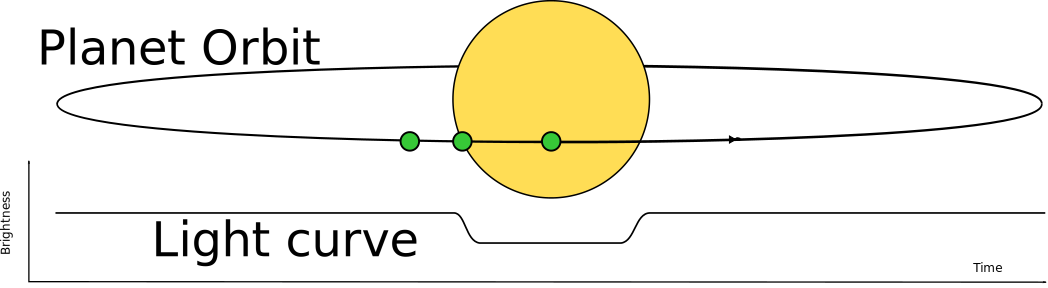
\includegraphics[width=0.8\textwidth]{images/planetary_transit.pdf}
    \caption{Example of simple model of planetary transit and the expected light curve}
    \label{fig:transit}
\end{figure}

By observing the flux from a star over period of time, any orbiting planet that passes in front of the star will cause a slight dip in the observed flux. This change in the light curve allows one to calculate the relative sizes of the planet and the star.

\paragraph{Advantages:}
\begin{itemize*}
    \item Easy to Perform
    \item Can be done at optical wavelengths
    \item Planet size can be determined
    \item Information about the planet's atmosphere can be obtained \citep{fortney2006atmosphere}
\end{itemize*}

\paragraph{Disadvantages:}
\begin{itemize*}
    \item Only works if orbital plane is in line with observer
    \item High false detection rate \citep{santerne2012sophie}
    \item Poor results for red giant stars due to their variable surface brightness
\end{itemize*}

As well as determining properties of the planet from the transit, by examining the regularity of these transits it is possible to determine information about other planets in the system. This is known as the transit timing variation method.

The period ($T$) of the planetary orbit can be figured out trivially by looking at the time between light curves. However large quantities of observations need to be taken for this.

Unfortunately the transit method only works well for large planets, as the flux dip is related to the square of the ratio of the planet to star radii. For instance observing a transit of the Earth from outside our solar system would only produce a fractional drop in flux of the order of $10^5$. A small drop like that would easily be hidden within the error, which is typically of the order of $10^3$ to $10^2$, and similar to a flux drop that would be observed simply due to a large Sunspot.

Using a simple uniform disk model (described in detail later), the planet radius can be obtained as:
\[ \frac{\Delta F}{F} = \left( \frac{R_p}{R_*} \right)^2 \]
\[ \Rightarrow R_p = R_* \sqrt{\frac{\Delta F}{F}} \]

\subsubsection{Radial Velocity}

Normally we talk about planets orbiting around a star, as this model approximates what we see very well. In actual fact however, the planet and star both orbit their common center of mass. Generally this center of mass is located very close to the center of the star so the, planet orbit model works well. However the star will move slightly, and is especially noticeable for very large planets orbiting closely, so called Hot Jupiters. As the star is moving in its own orbit, small doppler shifts can be seen in the spectrum of the star. Modern spectrometers are so accurate, that even small velocities of the order of $1\units{ms^{-1}}$ can be observed \citep{ge2002externally}. Observing using this method is often called 'Doppler Spectroscopy'.

\paragraph{Advantages:}
\begin{itemize*}
    \item Works well for low mass stars
    \item Distance independent
    \item Works for larger inclination range than transit method
    \item Gives orbital radius and planetary mass
\end{itemize*}

\paragraph{Disadvantages:}
\begin{itemize*}
    \item Depends on inclination
    \item Requires high signal to noise ratio of data
    \item Requires spectrometers rather than just CCD cameras
    \item Poor results for stars with fast rotational velocities
\end{itemize*}

The radius of orbit can be calculated as:
\[r^3 =\frac{GM_*}{4\pi^2}P_*^2 \]

Which gives the orbital velocity from Newtonian mechanics as:
\[v_p =\sqrt{\frac{GM_*}{r}} \]

The planetary mass can be calculated from the radial velocity as:
\[ m_P = \frac{M_*v_*}{v_P} \]

\subsubsection{Pulsar timing}

Pulsars rotate very rapidly, and emit radio waves as they do. The regularity of these emission is so precise that even tiny variations can be used to track the motion of the neutron star. In fact the first ever extra solar planet was confirmed using exactly this method in 1992 \citep{wolszczan1992planetary}. While this method is great for finding planets, these systems are quite rare. Also, due to the special conditions required to form planets around a white dwarf, and the intense radiation emitted, life as we know it could not evolve in these systems.

\subsubsection{Direct Observation}

\begin{figure}[ht]
    \centering
    \includegraphics[width=\figwidth]{images/direct_image.png}
    \caption{Direct image of 2MASS J01033563-5515561ABb, sourced from \cite{delorme2013direct}. The green arrow shows the position of the companion, and the blue circle shows where a background source would be expected.}
    \label{fig:direct}
\end{figure}

Under the right conditions, it can be possible to now see exoplanets directly \citep{lafreniere2010directly,kuzuhara2013direct,delorme2013direct}. Obviously stars are very bright compared to their orbiting planets making this technique a bad choice for discovering earth like planets. However large planets, many times the mass of Jupiter are observable. Using a coronagraph on the telescope limits the light from the star \citep{kuchner2002coronagraph}, and observing at infra red wavelengths can overcome the relative brightness problem \citep{delorme2013direct}.

\subsection{Selection Bias}

For all of the methods discussed, they generally favour finding large planets. This obviously leads to large selection bias in our current list of known exoplanets. While planets have proven to be commonplace in the universe, our sampling doesn't provide an overall dataset that can be used to draw conclusions about how planets are generally distributed, and if planetary systems like our own are rare or very common. This is discussed further in \citep{wright2011exoplanet}. The Kepler mission however was designed to search specifically for Earth like planets, so hopefully we will have a more comprehensive planetary database in the near future.

\section{Aims and Objectives}
\begin{itemize}
\item Create a computer software to simulate the change in observed flux from a planetary transit.
\item Observe known transits from the rooftop observatory, perform all the necessary data reduction and show that it is possible to perform useful observations even with the poor seeing in Cardiff.
\item Create a computer software that performs automated aperture photometry of stars, and use this with any observational data collected.
\item Use any observations obtained and the software pipeline constructed to infer properties of the transiting planets.
\end{itemize}


\section{Model}
%!TEX root = project.tex
Model using formulae from \cite{mandel2002analytic} and constants from \cite{mohr2012codata}


%\bibliographystyle{apj}
\bibliography{references}

\end{document}
